\chapter{Procedural Maze Generation} \label{procedural}
\begin{figure}[!h]
\centering
    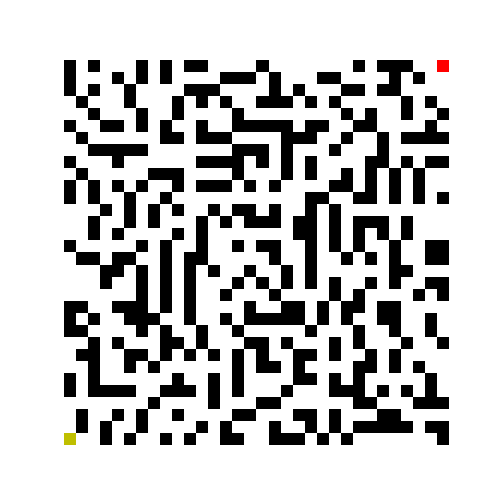
\includegraphics[width=.4\textwidth]{images/maze_example.png}
    \caption{Example maze generated by our program. Base CA: B1/S2345, Bias $\lambda$ = 0.6}
\label{fig:maze-example}
\end{figure}
We build an evolutionary algorithm toolkit to evolve life-like CA for procedural generation. Maze generation is picked as an appropriately challenging domain since the quality of a maze is dictated by global properties which cannot be directly encoded in the local interaction behaviour of CA. To generate a good maze, a CA rule must induce the birth and survival of cells at times that increase the likelihood of corridor and junction-like structures forming. Mazes bear many structural similarities to life-like CA including a lattice shape and two mutually-exclusive states, \textit{wall} and \textit{path}. Furthermore, two mazes with similar global properties tend to be phenotypically alike which simplifies evolutionary learning. However, CAs are stochastic systems and provide no guarantees that any maze generated will be solvable. To mitigate this, we implement a repair mechanism that amends near-valid solutions and discards solutions that do not meet a minimum criterion. This allows genes that contribute to high quality solutions to survive while maintaining a level of selection pressure on solution validity alongside solution quality.\\

This goal has some similarities to a work by C. Adams\cite{adams2018evolving} which also looks at the application of CAs in maze generation. However, this application differs notably from Adams' in both the evolution algorithm and fitness function design. Key features in our maze generator include the notion of failed rules, the stochastic region merging algorithm, and automated loss calculation (i.e. no external human input required to rank mazes).\\

The EA toolkit is written entirely in Python making use only of basic data manipulation and scientific computing libraries such as NumPy, SciPy, and Pandas as well as media libraries like Matplotlib and Python Imaging Library. It features the following key classes:
\begin{itemize}
    \item Experiment Suite: Includes methods and configurations for running evolutionary experiments.
    \item Population: Handles population-wide actions like crossover, elitism, and selection. It also tracks metrics for hyperparameter tuning.
    \item Chromosome: Handles individual actions like mutation, and fitness calculation.
    \item Simulator: Runs binary-state cellular automata, performs repair, and caches state data when needed
\end{itemize}
Each time we learn a new class of CA or optimise for a new objective, we write a new instance of the Population,  Chromosome, and Simulator classes.

\section{Simulator} \label{subsec:simulator}
Due to the undecidability of various CA rules, the state of an automaton after some time cannot, in general, be calculated without simulating each transition in turn. For this, a CA simulator was built.\\

The simulator stores the state of a 2D square CA of side length $N$ in an $N \times N$ NumPy array. The CA is initialised with birth set $B$ and survival set $S$ which are given as direct arguments or calculated from the chromosome as shown in \ref{eq:bs-calc}. When simulating $n$ time steps, the simulator begins by caching the current state $X^{(t)}$. Then a neighbourhood matrix $M$ is calculated by convolving $X^{(t)}$ with kernel $\kappa$ where
\[
    \kappa = \begin{bmatrix}
        1 & 1 & 1\\
        1 & 0 & 1\\
        1 & 1 & 1
        \end{bmatrix}    
\]
The value $M_{i,j}$ is the number of live neighbours of $X^{(t)}_{i,j}$. The convolution is calculated with wrapped boundaries to simulate periodic boundary conditions. The next state is calculated as follows
\[
    X^{(t+1)}_{i,j}= (\lnot X^{(t)}_{i,j} \land n \in B) \lor (X^{(t)}_{i,j} \land n \in S)
\]
where the left conjunction corresponds to the case of a dead cell becoming alive and the right conjunction corresponds to a living cell surviving. If $X^{(t+1)} = X^{(t)}$, the cached state, then no further steps are calculated since $X^{(t + n)} = X^{(t + n - 1)} = ... = X^{(t)}$ by induction. Otherwise, the current state is cached and the simulator continues until $n$ steps have elapsed or a later fixed point is reached. The simulator does not automatically detect periods of length greater than 1 as this would involve maintaining and comparing against a large history of previous states which would be too computationally intensive. The simulator allows the initial state $X^{(0)}$ to be set randomly with a particular density or to be set explicitly. It also saves CA states at regular intervals as images which are concatenated together into animated gifs.\\

\begin{figure}[!h]
\centering
            \subfloat[$t=0$]{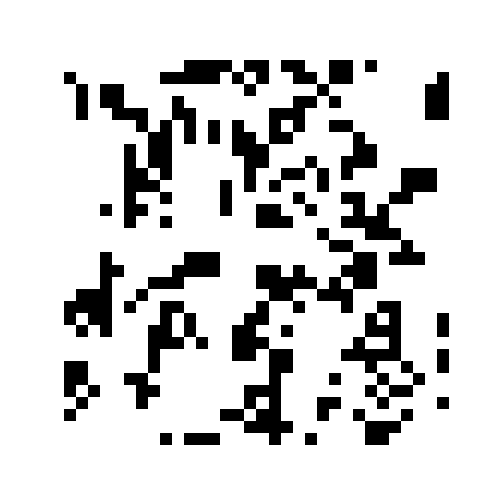
\includegraphics[width=.2\textwidth]{images/stains/0.png}}\hfill
            \subfloat[$t=1$]{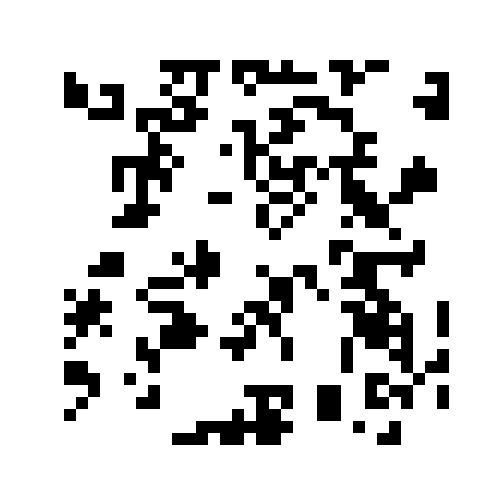
\includegraphics[width=.2\textwidth]{images/stains/1.png}}\hfill
            \subfloat[$t=2$]{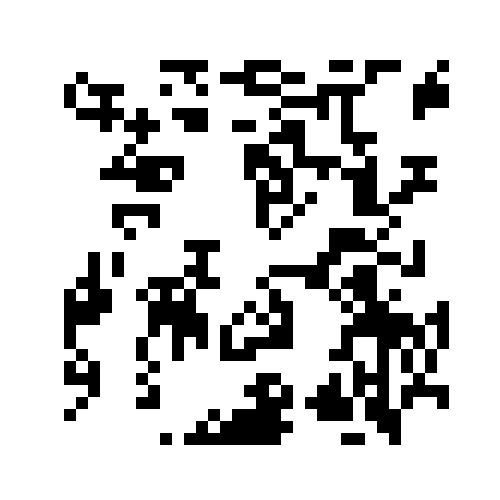
\includegraphics[width=.2\textwidth]{images/stains/2.png}}\hfill
            \subfloat[$t=3$]{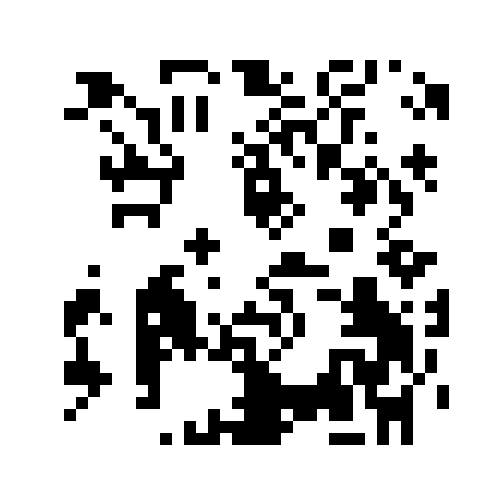
\includegraphics[width=.2\textwidth]{images/stains/3.png}}\hfill
            \subfloat[$t=4$]{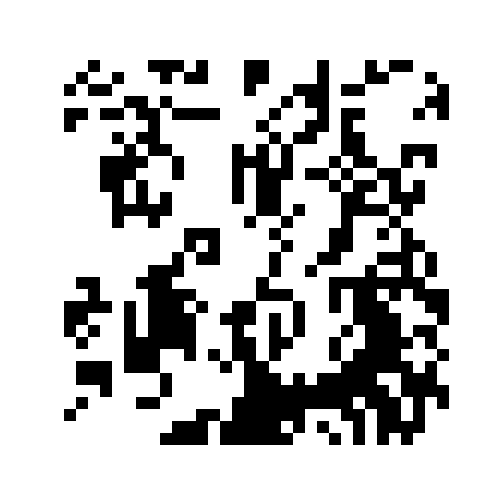
\includegraphics[width=.2\textwidth]{images/stains/4.png}}\hfill
            \caption{5 consecutive snapshots created in the simulator class of \textit{Stains}, a stable rule with rulestring B3678/S235678}
\label{fig:stains}
\end{figure}

\section{Procedural Generation}
A maze is generated from a chromosome in three stages: growth, region search, and region merging. During the growth stage, a CA is run in the simulator for a fixed number of iterations, typically 50, using the birth and survival sets encoded in the chromosome. 

\subsection{Region Search}

The region search stage uses randomly initialised breadth first searches to find all disconnected regions within the maze. In order to perform the merge stage later on, two data structures are populated during the search stage. The first is a hashmap from each cell to the region number of the region it occupies. The second is the reverse, a hashmap from each region number to the set of cells in that region.

\begin{algorithm}
  \caption{Region Search Algorithm}\label{alg:region-find}
  \begin{algorithmic}
  \Require $X$ - the state of the CA after the growth stage
  \Ensure cells[($c_x$, $c_y$)] = $r_c \iff$ ($c_x$, $c_y$) $\in$ regions[$r_c$]

  \Comment{Initialisation}
  \State cells $\gets$ empty dictionary of type \{(int, int): int\}
  \State regions $\gets$ empty dictionary of type \{int: set\{int\}\}
  \State spaces $\gets$ set of cells in X with state 0

  \Comment{Find first region}
  \State $r_1 \gets$ \Call{BFS}{start-cell, $X$}
  \State \Call{UpdateDicts}{$r_1$, 1}
  
  \Comment{Find remaining regions}
  \State counter $\gets 1$
  \While{spaces not empty}
    \State counter $\gets$ counter + 1
    \State startCell $\gets$ randomly chosen 0-state cell
    \State $r \gets$ \Call{BFS}{startCell, $X$}
    \State \Call{UpdateDicts}{$r$, counter}
  \EndWhile

  \Comment{Update Function}
  \Procedure{UpdateDicts}{region, index}
    \For{$c$ in region}
        \State cells[$c$] = index
        \State regions[index].add($c$)
    \EndFor
    \State spaces $\gets$ spaces - $r$
  \EndProcedure
  \end{algorithmic}
\end{algorithm}



\subsection{Region Merge}

The region merge stage connects regions randomly until a connected path exists from the start cell to the goal cell or the maze is deemed invalid. It is crucial for the region merging algorithm to be stochastic. If it is deterministic and merges regions according to a pre-designed pattern, the genetic algorithm is incentivised to learn rules that lend themselves well to this pattern. For example, if mazes with longer solution paths are considered fitter and the merging algorithm connects regions in horizontal bands sweeping left-to-right (as in \cite{adams2018evolving}) then the evolutionary process is incentivised to produce rules with shorter horizontal corridors over longer vertical corridors. This is in direct conflict with the fitness function. To avoid this, we design a stochastic region merging algorithm. It begins with the region containing the start cell. Each wall cell bordering this region is examined to determine whether removing the cell would connect to a distinct region. One of these wall cells is randomly chosen and removed. This process repeats on the union of the two joined regions. If no such wall cells exist, the simulation is deemed invalid. This can be thought of as only permitting walls of width 1 to be broken when connecting regions. Allowing walls of arbitrary thickness to be joined is undesirable as it diminishes the contribution of the CA over the final solution. Consider the extreme case of a maze with only walls except the start and end goal. If the merging algorithm connects these two cells, the solution's form is a consequence of the merging algorithm alone and not the CA which generated a maze of walls in the first place. This would clearly be undesirable. If a chromosome does not yield a minimum percentage of valid simulations, it is assigned a fitness of 0 and usually removed from the population in the following iteration.

\begin{algorithm}
  \caption{Region Merge Algorithm}\label{alg:region-merge}
  \begin{algorithmic}
  \Require cells, regions, X
%   \Ensure cells[($c_x$, $c_y$)] = $r_c \iff$ ($c_x$, $c_y$) $\in$ regions[$r_c$]
  \State visited $\gets$ regions[1]
  \While{True}
    \State fringe $\gets$ \Call{OneNeighbours}{visited}
    \If{goalCell in fringe}
        \State return True \Comment{Success}
    \EndIf
    \State candidates $\gets$ []
    \For{$f$ in fringe}
        \State zeros $\gets$ \Call{ZeroNeighbours}{$f$}
        \If{length(zeros - visited) > 0}
            \State candidates.append($f$)
        \EndIf
    \EndFor
    \If{length(candidates) > 0}
        \State $c \gets$ \Call{PopRandom}{candidates}
        \State visited.add($c$)
        \State X[$c$] = 0
        \State newRegions $\gets$ \{cells[$d$] for $d \in$ \Call{ZeroNeighbours}{$c$}\}
        \State visited $\gets$ visited $\cup$ \{regions[$r$] for $r \in$ newRegions\}
    \Else
        \State return False \Comment{Failure}
    \EndIf
  \EndWhile
  \State
  \State where \Call{OneNeighbours}{} and \Call{ZeroNeighbours}{} return the 1-state and 0-state neighbours of a cell respectively.
  \end{algorithmic}
\end{algorithm}
\todo{Image of merge}

\section{Genetic Algorithm I}\label{sec:ga-1}

A genetic algorithm is used to evolve a population of chromosomes that represent the transition rule of the life-like CA.

\subsection{Chromosome}
A transition rule can be represented in a number of ways. Most intuitively, consider a birth and survival set indicating the number of neighbours that elicit a dead cell to become alive or a living cell to remain alive respectively. This can be encoded as a binary string or in integer form as shown in equation~\ref{eq:bs-calc}.

\begin{equation} \label{eq:bs-calc}
\begin{split}
    \text{Number of neighbours:}&\ 0\ 1\ 2\ 3\ 4\ 5\ 6\ 7\ 8\ |\ 0\ 1\ 2\ 3\ 4\ 5\ 6\ 7\ 8\\
    \text{Binary representation:}&\ 0\ 0\ 0\ 1\ 0\ 0\ 0\ 0\ 0\ |\ 0\ 0\ 1\ 1\ 0\ 0\ 0\ 0\ 0\\
    &\qquad\ \: \uparrow \qquad \qquad \qquad \ \: \: \uparrow \ \uparrow\\
    \text{Set representation:}&\quad \ \text{B:} \{3\} \qquad \qquad \ \ \: \text{S:}\{2, 3\}\\
    \text{Integer representation:}&\ \texttt{0b000100000001100000} = 16480
\end{split}   
\end{equation}

Each binary string chromosome has length 18, so the discrete search space is of size $2^{18} = 262144$. An initial population of $\mu$ chromosomes is chosen randomly from a distribution that is uniform over the density of the binary representations. As shown by [CITE], this is preferable to a distribution that is uniform over the integer representations since the density of the rule is more correlated with complexity properties than the integer value of the rule [EVIDENCE]. When initialising a random chromosome, a density $\rho$ is picked uniformly from $[0.0, 1.0]$. Then, each bit is a sample from the $\mathit{Bernoulli}(\rho)$ distribution.\\

\subsection{Genetic Operators}
At each iteration, the algorithm explores the search space through a collection of genetic operators. Crossover and mutation produce novel candidates, fitness functions evaluate each individual, and selection concentrates learned information in a set of elite parents. In accordance with the $\frac{1}{5}$ rule \todo{explain and cite this}, we produce $\lambda$ new children in each expansion stage and reduce down to $\mu$ elite candidates in each contraction stage with $\lambda \approx 4\mu$. Single-point crossover is used to produce new children. Pointwise mutation is applied with probability $\frac{1}{18}$ such that the expected number of bit flips per chromosome is 1. For efficiency, this is actually implemented by generating a mutation mask with expected density $\frac{1}{18}$ and applying XOR between the chromosome and mutation mask.\\

When producing the next generation we consider selection criteria based on fitness and age. In a $(\mu + \lambda)$ selection setting, we produce a population of $\lambda$ children from $\mu$ parents and the next generation is selected from the collective. In a $(\mu, \lambda)$ setting, the next generation is selected exclusively from the $\lambda$ children. We can interpret this as an age restriction of 1 generation on the $\mu$ parent candidates. Common forms of selection include roulette and truncation. In truncation selection, all candidates are linearly ranked by fitness and the top $\mu$ candidates progress to the next generation. In roulette selection, the probability of each individual progressing to the next generation is proportional to its objective fitness. Both are implemented and compared in Chapter\ref{evaluation}\\

\subsection{Fitness Function}
The aim of the fitness function is to assess the maze using quantitative metrics that can be calculated efficiently. For example, the number of vacant cells reachable from the start cell is an important metric because, if this is too low, a large portion of the maze is wasted space. This metric is computed in linear time with respect to the number of cells in the automata by performing a breadth first search in the region containing the start cell and recording the number of vacant cells in the maze that exist outside this region. We opt for two metrics: the number of dead ends and the solution path length. A cell is considered to be a dead end if all its neighbours are wall cells or vacant cells that have already been visited. These two factors work well as they are easy to calculate, well-correlated with perceived maze difficulty[CITE] and, crucially, oppose each other. A maze with a long solution tends to have long corridors whereas a maze with many dead ends tends to have shorter corridors and more decisions to make at each junction. By optimizing on conflicting objectives, we automatically regulate learning speed and reduce the probability of premature convergence to local optima. Assuming a maze with at least one solution, both metrics can be calculated simultaneously in a single breadth-first search traversal.\\
\todo{Image of algorithm finding num dead ends}
Initially, the fitness function $f(c_i) = s + \lambda d$ where s is the solution path length and d is the number of dead ends, was considered. However, this is not normalized as the solution length and number of dead ends are not on the same scale. Moreover, we cannot normalize each metric individually based on the range of values present in a given generation since the ranges vary from experiment to experiment and generation to generation. Instead, a truncated linear selection is performed with fitness function $f(c_i) = r_s + \lambda r_d$ where $r_s$ and $r_d$ are the rank of the cell in the population according to solution length and number of dead ends respectively.